\chapter{Computer Vision Evaluation}
\label{ch:cveval}
% Source: docs/fyp2-plan/CV_EVAL_CHAPTER.md (B6 results sheet). Every number below names the file or command it comes from.
% Reports live in backend/interaction/benchmarks/ unless stated otherwise.

This chapter reports how well the vision pipeline detects people, tells employees from customers, finds customer--employee interactions and runs on commodity hardware. It separates numbers measured on clips the rules were tuned on from numbers measured on clips held out from tuning, gives confidence intervals for the headline figure, and explains every error on the held-out set. All speed figures are CPU only.

\section{Evaluation Design}
\label{sec:cveval-design}

\subsection{Datasets and Splits}
The interaction benchmark uses 25 labelled clips from one store and two cameras, split into two sets:
\begin{itemize}
\item \textbf{Tuning set (11 clips)}, \path{benchmark.json}: 13 labelled interactions and 4 pass-bys. The interaction rules were tuned on these clips, so their scores are optimistic.
\item \textbf{Set B (14 held-out clips)}, \path{benchmark_set_b.json}: 17 labelled interactions and 9 pass-bys. This is the headline set. It was looked at once during tuning, to set the span-merge rule, and is otherwise unseen.
\end{itemize}
Together the sets hold 30 labelled interactions (target 30) and 13 pass-bys (target 15). Labels were drafted and reviewed in CVAT and imported with \path{backend/interaction/cvat_import.py}. The tuning-set labels have a single annotator.

The detector training split is by recording (\path{split_manifest.csv}). Set B uses only test and validation recordings, so no set-B frame was seen in detector training; most tuning clips are training recordings. A provenance audit on 13 November corrected the set-B pass-by count from 10 to 9 and established that the earlier ``random six'' reports reuse four tuning clips and two set-B clips; they are therefore quoted only as a hand-set versus fitted roles comparison, never as an independent test.

For roles, every person in the 25 clips was reviewed (\path{persons.json}). A pipeline track takes the role of the reviewed person it overlaps most, provided the boxes overlap at IoU $\geq 0.3$ in at least half of the track's frames (\path{role_labels.py}); 109 of 113 tracks received a label this way.

\subsection{Metrics}
A predicted interaction matches a labelled one when their time spans overlap at temporal IoU $\geq 0.5$, with one-to-one matching; precision, recall and F1 follow from the matched counts. Because strict matching counts one long prediction covering several short labels as a miss plus a false alarm, a per-second overlap score is reported alongside it. Confidence intervals are clip-level bootstraps with 10\,000 resamples and seed 0. Commands:
\begin{itemize}
\item \texttt{python -m backend.interaction.benchmark <spec> --output <report>}
\item \texttt{python -m backend.interaction.confidence <report>}
\item \texttt{python -m backend.interaction.refit <spec>} (role weights, Section~\ref{sec:cveval-roles})
\end{itemize}

\section{Results by Stage}
\label{sec:cveval-results}
Table~\ref{tab:cveval-stages} gives each stage's result on both sets. The headline interaction result is F1~0.462 on set B with the pose judge, with a 95\,\% interval of 0.27--0.65.

\begin{longtable}{P{0.17\textwidth}P{0.15\textwidth}P{0.24\textwidth}P{0.2\textwidth}P{0.18\textwidth}}
\caption{Vision pipeline results by stage}\label{tab:cveval-stages}\\
\toprule
Stage & Metric & Set B (held out) & Tuning set (11) & Source\\
\midrule
\endfirsthead
\toprule
Stage & Metric & Set B (held out) & Tuning set (11) & Source\\
\midrule
\endhead
Detector (best\_320, OpenVINO, 455 test images) & mAP50 / mAP50--95 / P / R & 0.969 / 0.896 / 0.963 / 0.953 & same detector & \path{report_set_b_merged.json}\\
Interactions, proximity only & P / R / F1 & 0.360 / 0.529 / 0.429 (TP 9, FP 16, FN 8) & 0.619 / 1.000 / 0.765 & \path{report_set_b_merged.json}, \path{report_11_merged.json}\\
Interactions, with pose judge & P / R / F1 & \textbf{0.409 / 0.529 / 0.462} (TP 9, FP 13, FN 8) & 0.765 / 1.000 / 0.867 (TP 13, FP 4, FN 0) & same\\
F1 95\,\% CI, with judge & & [0.267, 0.645] & [0.788, 0.960] & \texttt{confidence}\\
F1 95\,\% CI, proximity only & & [0.245, 0.600] & [0.625, 0.917] & \texttt{confidence}\\
Per-second overlap, with judge & P / R / F1 & 0.521 / 0.943 / 0.671 & 0.711 / 0.904 / 0.796 & \texttt{overlap\_seconds} on the saved spans\\
Timing, with judge & start / end error (s) & 1.16 / 2.93 & 1.15 / 1.96 & reports above\\
Roles & accuracy per track & 1.000 (59 tracks, fitted weights) & & \path{report_set_b_roles_hand.json}\\
% NOTE (Ruhab): the results sheet attributes this roles run to fitted weights although the file name says "hand"; confirm with Saqib before submission.
Tracking & ID switches per minute & 1.82 & 2.29 & reports above\\
Speed & CPU realtime factor & \textbf{0.60$\times$} & & \path{report_set_b_speed_idle.json}\\
\bottomrule
\end{longtable}

\paragraph{Effect of the pose judge.} On set B the judge removes 3 of the 16 proximity-only false positives without losing a true positive, raising precision from 0.360 to 0.409 and F1 from 0.429 to 0.462. On the tuning set it removes half the false positives (8 to 4). Recall is unchanged on both sets because the judge only ever vetoes candidates.

\paragraph{Tuning set versus held-out set.} F1 falls from 0.867 to 0.462 between the tuning set and set B, and the two confidence intervals do not overlap. The gap is the expected cost of tuning rules on a small set and is the main reason set B is the headline. Recall on set B is 0.529, and the per-second recall of 0.943 shows that most labelled interaction time is covered by some prediction: the pipeline usually finds the pair but draws the span boundaries differently from the labeller (Section~\ref{sec:cveval-errors}).

\paragraph{Speed.} On an idle machine with nothing else running, the current pipeline processes set B at 0.60$\times$ realtime on CPU (frame median about 95\,ms; the pose judge takes 240--320\,ms per call), and up to about 1.5$\times$ on individual clips. The 0.87$\times$ figure measured on 7 November predates the merge of the shared code. Runs that shared the CPU with other work (0.09--0.48$\times$) are not valid speed measurements and are not reported. The rerun on the idle machine reproduced F1~0.462 exactly. GPU throughput was not measured.

\section{Role Weights}
\label{sec:cveval-roles}
Each track's role comes from a weighted sum of employee-evidence factors compared with a threshold (\path{cust_emp_classifier.py}). The hand-set weights are reference 0.55, bib colour 0.30, staff zone 0.10, stationary 0.05, threshold 0.45; on uncalibrated cameras the reference weight passes to the role model's own class. A logistic regression fitted with leave-one-clip-out validation was compared with these weights on held-out clips (Table~\ref{tab:cveval-roles}).

\begin{table}[H]
\centering
\caption{Hand-set versus fitted role weights (leave-one-clip-out)}
\label{tab:cveval-roles}
\begin{tabular}{P{0.2\textwidth}P{0.15\textwidth}P{0.2\textwidth}P{0.13\textwidth}P{0.24\textwidth}}
\toprule
Set & Hand-set accuracy & Hand-set employee recall & Fitted accuracy & Source\\
\midrule
Tuning set (50 tracks) & 0.960 & 0.889 & 1.000 & \path{refit_benchmark/refit.json}\\
Set B (59 tracks) & 0.915 & 0.815 (misses 5 of 27) & 1.000 & \path{refit_benchmark_set_b/refit.json}\\
\bottomrule
\end{tabular}
\end{table}

Fitted on the tuning set alone and scored on set B, the fitted weights classify all 59 tracks correctly. The fit puts nearly all weight on the role model's class (0.61) and bib colour (0.36), a little on standing still (0.02--0.03), and none on reference similarity or staff zones, with a threshold of 0.07--0.09 (\path{store_roles_fitted.json}). The zero weights mean these factors were never observed in the clips, since no camera is calibrated and no staff zone is drawn; they do not mean the factors are useless. Figure~\ref{fig:role-sweep} shows that the fitted weights keep full employee recall over a wide band of thresholds, whereas the hand-set recall falls as soon as the threshold passes about 0.2.

\begin{figure}[htbp]
\centering
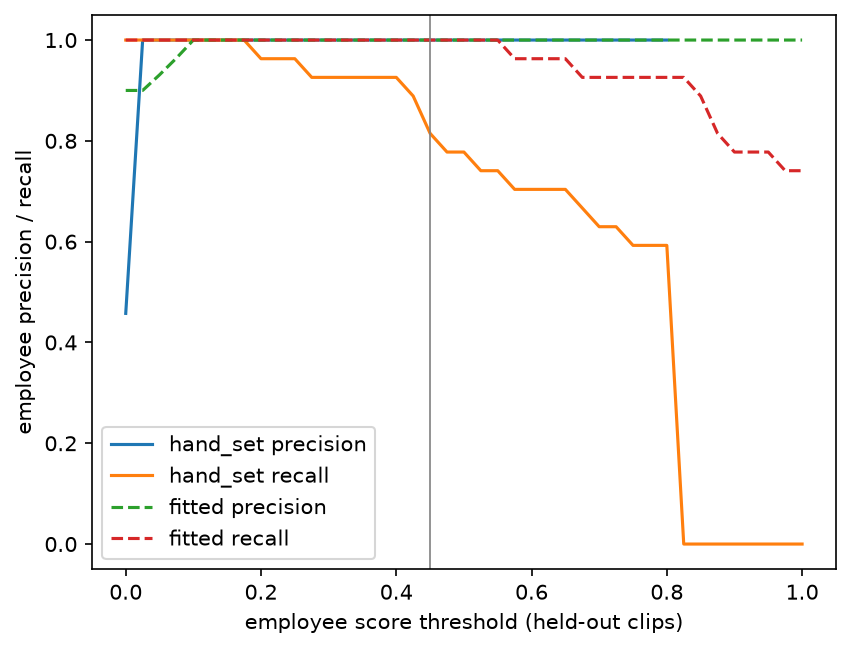
\includegraphics[width=0.7\textwidth]{ThesisFigs/role_threshold_sweep_set_b.png}
\caption{Employee precision and recall against the score threshold on held-out set-B clips, hand-set (solid) and fitted (dashed) weights. The grey line marks the hand-set threshold of 0.45.}
\label{fig:role-sweep}
\end{figure}

\paragraph{Decision (B3).} The fitted weights ship. They miss no employee on held-out data, where the hand-set weights miss 5 of 27, and their low threshold keeps employee recall stable over a wide range rather than at a single tuned point. The weights are a per-store configuration, so a store whose cameras are calibrated or have staff zones refits them rather than inheriting these values. With two cameras and few clips, the 100\,\% figure is not a general accuracy claim. Both benchmark specifications now load the fitted configuration for every clip, and the benchmarks are rerun with it before the model freeze.

\section{Signals in the Event Store}
\label{sec:cveval-signals}
Every pipeline run is written to PostgreSQL by \path{backend/events/ingest.py} (schema v1) and checked by a contract test (\path{backend/events/test_events.py}) on both the fixture day and real CV runs.
\begin{itemize}
\item \textbf{Measured on real footage:} interactions, per-track roles, unattended-customer episodes, pipeline health (frame rate, confidence, unknown-role share, ID churn, frozen or dark frames) and one people heatmap per camera per hour, not split by role.
\item \textbf{Fixture only until the store map is registered:} named-zone dwell and transitions, entrance-line footfall, and queue length and wait. These are validated by unit tests against planted fixture patterns, not against labelled footage, because no camera has zone polygons yet.
\end{itemize}
Unattended-customer episodes reach direct dispatch automatically (\path{backend/dispatch.py}).

Camera handoff (\texttt{python -m backend.handoff\_eval}) is implemented and unit-tested but not evaluated, because no cross-camera crossings are labelled.

\section{Error Analysis}
\label{sec:cveval-errors}
All 13 false positives and 8 misses on set B (with judge, \path{report_set_b_merged.json}) were inspected frame by frame. They fall into three groups.
\begin{enumerate}
\item \textbf{Span too long (4 false positives, 6 misses).} One prediction covers several shorter labelled interactions; for example, a prediction from 9.7\,s to 38.3\,s on clip 155639 covers labels at 11.2--15.8, 19.5--28.4 and 34.3--36.7\,s. The 4\,s gap bridge and the span merge join interactions that the labeller kept apart. The pair is found correctly; what is open is the convention for a pause of 4--6\,s. This group explains most of the gap between strict F1 (0.462) and per-second F1 (0.671).
\item \textbf{Duplicate after a customer ID switch (4 false positives).} When the tracker gives a customer a new ID mid-interaction, the same-customer merge cannot join the two halves. The fix belongs in tracking or re-identification, not in the merge rules.
\item \textbf{No label nearby (5 false positives).} Two look like missed labels: on IMG\_8838 part 2 the pair stand face to face for about 28\,s, and on IMG\_8830 a customer gestures at a seated employee. One is a genuine false positive where two employees talk (a role flip or a nearby customer), and two are probably genuine false positives where people stand side by side without engaging.
\end{enumerate}
If a blind re-check confirms the two suspected missed labels, set-B precision becomes about 0.455, recall 0.526 and F1 0.488. Until that re-check is done, the reported figure stays 0.462.

\section{Limitations}
\label{sec:cveval-limits}
\begin{itemize}
\item \textbf{Small labelled set:} 30 interactions in 25 clips from one store and two cameras. The 95\,\% interval on set-B F1 spans 0.27--0.65.
\item \textbf{One look at set B:} set B was used once during tuning, to set the span-merge rule.
\item \textbf{Tracking:} customer ID switches (1.8 per minute on set B) cause duplicate spans; no tracking fix was made.
\item \textbf{CPU only:} at 0.60$\times$ realtime, the demonstration runs on recorded footage rather than live streams.
\item \textbf{No zone geometry:} zone-level signals are validated on fixtures only.
\item \textbf{Single annotator:} the tuning-set labels have no second annotator, and pass-bys are judgement calls.
\item \textbf{Role weights:} the fitted weights were learned and tested on two uncalibrated cameras; they must be refitted for other stores.
\end{itemize}
